
\section{Experiments}
\label{sec:experiments}

\boldparagraph{Experimental setup.} In this study, we evaluate our method on COCO~\cite{lin2014mscoco}, a commonly used dataset for object detection, instance segmentation, and panoptic segmentation tasks. By default, we use plain features with adaptive-scale attention as described in \cref{sec:simplr} due to its strong performance and ability to perform both detection and segmentation; and initialize the ViT backbone from MAE~\cite{he2022mae} pre-trained on ImageNet-1K without any labels. In both fixed-scale and adaptive-scale attention, we set the number of scale $m=4$ and the window size $s=32$. Unless specified, the hyper-parameters are the same as in \cite{nguyen2022boxer}.

For all experiments, our optimizer is AdamW~\cite{loshchilov2019adamw} with a learning rate of 0.0001. The learning rate is linearly warmed up for the first 250 iterations and decayed at 0.9 and 0.95 fractions of the total number of training steps by a factor 10. ViT-B~\cite{dosovitskiy2021vit} is set as the backbone. The input image size is $1024\times1024$ with large-scale jitter \cite{shiasi2021lsjitter} between a scale range of $[0.1, 2.0]$. We employ query denoising~\cite{zhang2023dino} when compared with other methods. Due to the limit of our computational resources, we report the ablation study using the standard $5\times$ schedule setting with a batch size of 16 as in \cite{nguyen2022boxer}. In the main experiments, we use the finetuning recipe from \cite{li2022vitdet}.

% \boldparagraph{A single-scale detector is non-trivial.} We first study the effect of the scaling transformation in box-attention on feature pyramids as it could possibly generate regions-of-interest at different scales. More specifically, we compare the area between generated regions and the initial reference window of query vectors corresponding to object proposals in the last encoder layer. Surprisingly, the change of area after scaling has a mean of 31\% and standard deviation 33\% \wrt the original area of the reference window (\eg, for a reference window of $32\times32$ pixels to capture regions of different scales, such as $64\times64$ or $16\times16$ pixels, the change of the area should be more than 75\%). This suggests that the scaling function in box-attention prefers to capture regions of different aspect ratios rather than multi-scale information. 

% It can be seen in \cref{fig:single_scale} that deploying feature pyramids brings a large improvement to different types of detectors (\ie, $\sim$2 AP points for BoxeR and $\sim$3 AP points for ViTDet). This observation is consistent to the observation in DeformableDETR \cite{zhu2021deformable} where the improvement of $\sim$2 AP points comes from feature pyramids. While removing multi-scale input to the detection head, the PlainDETR~\cite{lin2023plaindetr} still depends on features pyramids to generate object proposals, their performance drops by $\sim$1 AP when using single-scale features for proposal generation.

\begin{table}[t]
    {
    \centering
    \footnotesize
    {
    \tablestyle{6pt}{1.2}
    \begin{tabular}{lccc}
    \multicolumn{1}{l|}{} & \multicolumn{1}{c|}{\multirow{2}{*}{FPS}} & \multicolumn{1}{c}{\multirow{2}{*}{AP$^\text{b}$}} & \multicolumn{1}{c}{\multirow{2}{*}{$\text{AP}^\text{m}$}} \\
    \multicolumn{1}{l|}{} &  \multicolumn{1}{c|}{} &  \multicolumn{1}{c}{} &  \\
    \shline
    \rowcolor{orange!50} \textbf{Feature pyramids} &  &  & \\
    \multicolumn{1}{l|}{DETR reported in~\cite{lin2023plaindetr}} & \multicolumn{1}{c|}{-} & 46.5 & n/a \\
    \multicolumn{1}{l|}{DeformableDETR reported in~\cite{lin2023plaindetr}} & \multicolumn{1}{c|}{12} & 52.1 & n/a \\
    \multicolumn{1}{l|}{DeformableDETR (our impl.)} & \multicolumn{1}{c|}{12} & 54.6 & n/a \\
    \multicolumn{1}{l|}{BoxeR~\cite{nguyen2022boxer}} &  \multicolumn{1}{c|}{12} & 55.4 & 47.7 \\
    \multicolumn{1}{l|}{ViTDet w/ Cascade head~\cite{li2022vitdet}} & \multicolumn{1}{c|}{11} & 54.0 & 46.7 \\
    \hline
    \rowcolor{orange!50} \textbf{Plain detector} &  &  & \\
    \multicolumn{1}{l|}{PlainDETR$^\dag$~\cite{lin2023plaindetr}} & \multicolumn{1}{c|}{12} & 53.8 & n/a \\
    \multicolumn{1}{l|}{{\ours}} & \multicolumn{1}{c|}{\bf 17} & {\bf 55.7} & {\bf 47.9}  \\
    \end{tabular}
    }
    \begin{tablenotes}
    \centering
    \item[] $\dag$: Multi-scale features are used to generate object proposals.
    \end{tablenotes}
    % \vspace{1em}
    {\caption{\textbf{\ours is an effective plain detector.} All methods use ViT-B as backbone. Methods that take feature pyramids as input employ SimpleFPN with ViT from \cite{li2022vitdet}. Our plain detector, \ours, shows competitive performance compared to multi-scale alternatives, while being faster during inference.}\label{tab:compare}}%
    }
\end{table}

\begin{table}[t]
    \begin{minipage}{\linewidth}
        \centering
        \footnotesize
        \subfloat[\label{tab:strat} \textbf{Scale-aware attention.}]
        {
        \tablestyle{5pt}{1.2}
        \begin{tabular}{l|cc}
        attention & AP$^\text{b}$ & $\text{AP}^\text{m}$ \\
        \shline
        base & 53.6 & 46.1 \\
        \hline
        i) fixed-scale & 55.0 & 47.2 \\
        \rowcolor{orange!25} ii) adaptive-scale & 55.4 & 47.6 \\
        & & \\
        \end{tabular}
        }
        \hspace{2mm}
        \subfloat[\label{tab:window_size} \textbf{Window size.}]
        {
        \tablestyle{5pt}{1.2}
        \begin{tabular}{l|cc}
        $s$ & AP$^\text{b}$ & $\text{AP}^\text{m}$ \\
        \shline
        base & 53.6 & 46.1 \\
        \hline
        16 & 55.1 & 47.4 \\
        \rowcolor{orange!25} 32 & 55.4 & 47.6 \\
        64 & 55.1 & 47.4 \\
        \end{tabular}
        }
        \hspace{2mm}
        \subfloat[\label{tab:num_scale} \textbf{Number of window scales}.]
        {
        \tablestyle{9pt}{1.2}
        \begin{tabular}{l|cc}
        $n$ & AP$^\text{b}$ & $\text{AP}^\text{m}$ \\
        \shline
        base & 53.6 & 46.1 \\
        \hline
        2 & 54.6 & 47.0 \\
        \rowcolor{orange!25} 4 & 55.4 & 47.6 \\
        6 & 55.2 & 47.6 \\
        \end{tabular}
        }

        \subfloat[\label{tab:feat_scale} \textbf{Scales of input features.}]
        {
        \tablestyle{6.5pt}{1.2}
        \begin{tabular}{l|cc}
        scale & AP$^\text{b}$ & $\text{AP}^\text{m}$ \\
        \shline
        base & 53.6 & 46.1 \\
        \hline
        1/4 & 55.4 & 47.7 \\
        \rowcolor{orange!25} 1/8 & 55.4 & 47.6 \\
        1/16 & 54.3 & 46.7 \\
        \end{tabular}
        }
        \hspace{5mm}
        \subfloat[\label{fig:attn_vis} Visualization of scale distribution learnt in \textbf{multi-head adaptive-scale attention} of object proposals. Objects are classified into \emph{small}, \emph{medium}, and \emph{large} based on their area.]
        {
        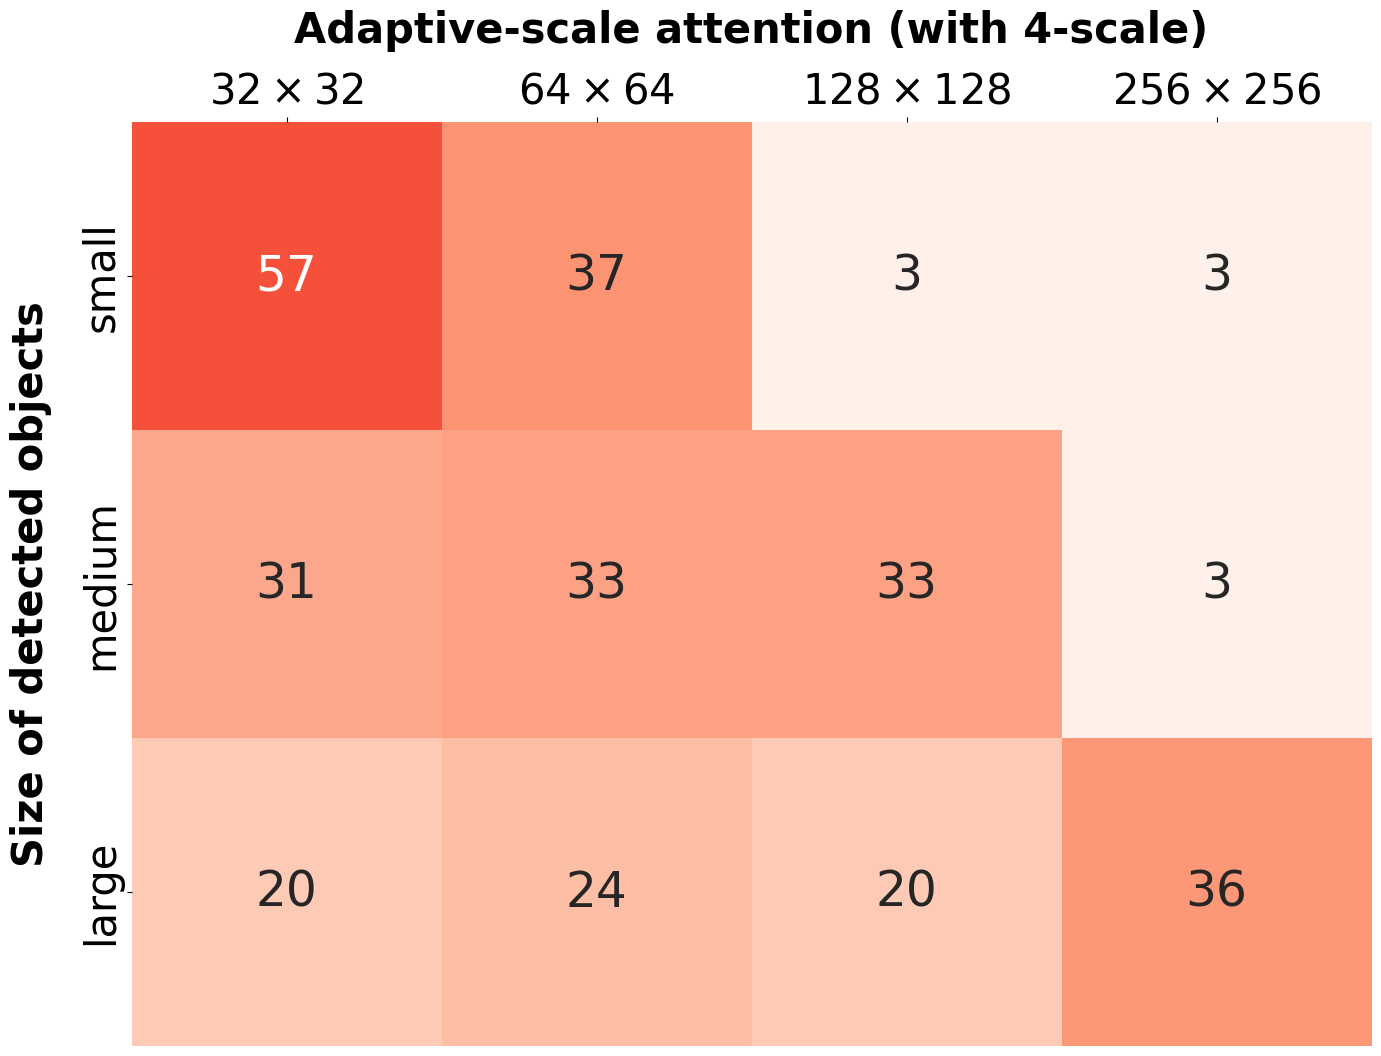
\includegraphics[width=0.46\textwidth]{fig/adaptive_scale.png}
        }
    \end{minipage}
    % \setcounter{table}{2}
    % \setcounter{subtable}{4}
    % \begin{minipage}{0.4\linewidth}
    %     \centering
    %     % \vspace*{1mm}
    %     \subfloat[\label{fig:attn_vis} Visualization of scale distribution learnt in \textbf{multi-head adaptive-scale attention} of object proposals. Objects are classified into \emph{small}, \emph{medium}, and \emph{large} based on their area.]
    %     {
    %     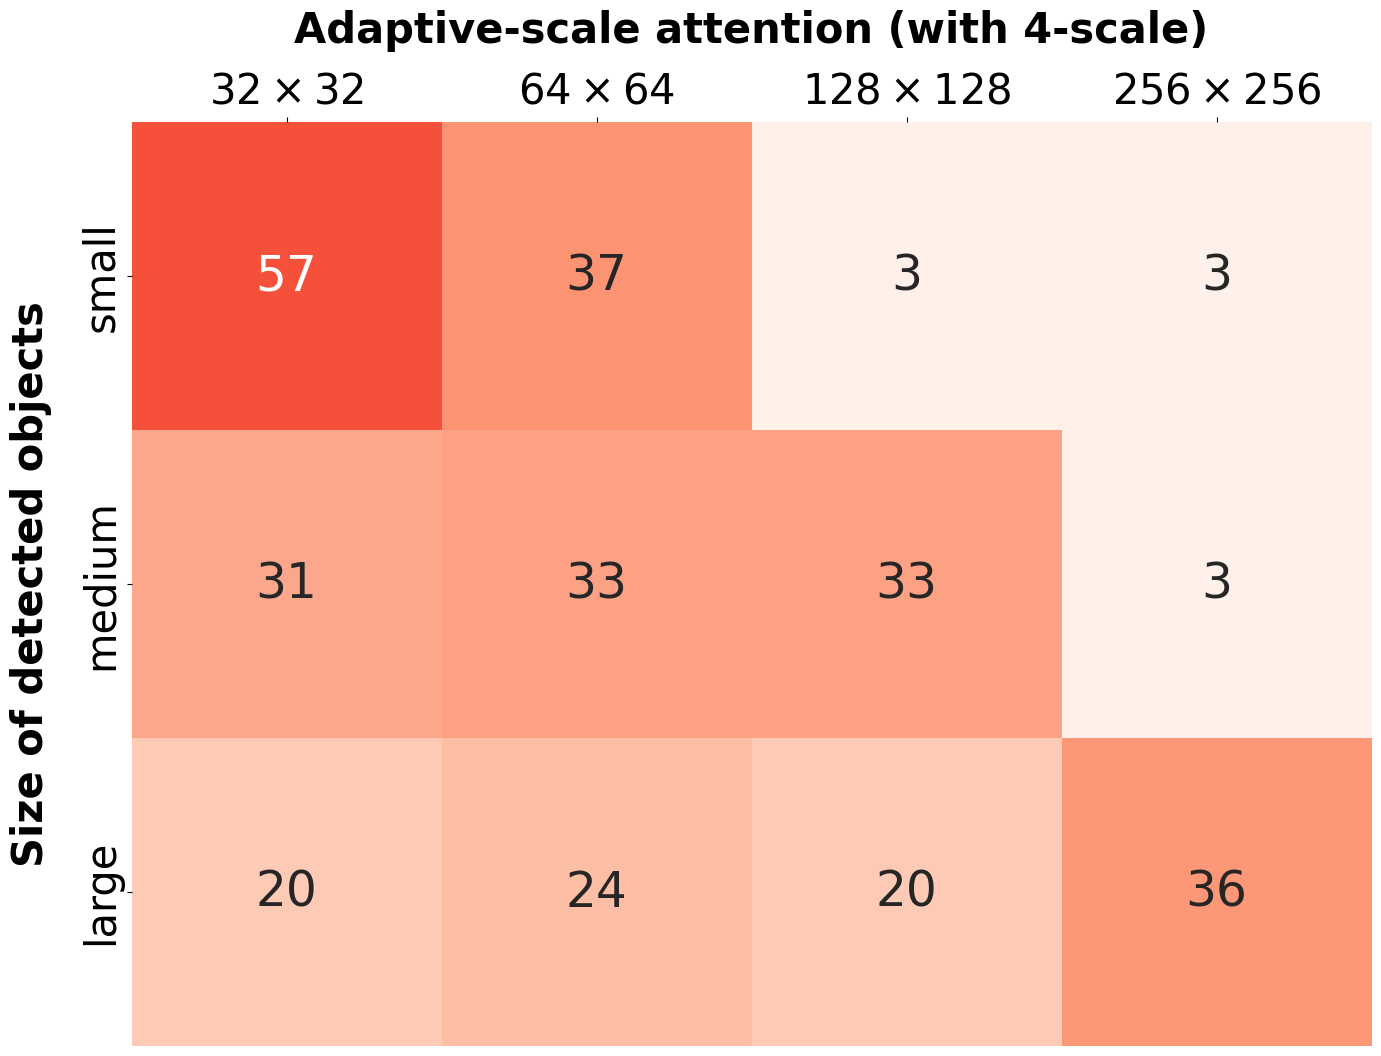
\includegraphics[width=\textwidth]{fig/adaptive_scale.png}
    %     }
    % \end{minipage}
    % \setcounter{table}{2}
    \caption{\label{tab:det_ablation} \textbf{Ablation of scale-aware attention} in \ours using a plain ViT backbone on COCO~\val. \textbf{Table (a-d):} Compared to the na\"ive baseline, which employs BoxeR and box-attention \cite{nguyen2022boxer} with \textit{single-scale} features, our plain detector, \ours, with scale-aware attention improves the performance consistently for all settings, default setting highlighted. 
    \textbf{Figure e:} our adaptive-scale attention captures different scale distribution in its attention heads based on the context of query vectors. Specifically, queries of \emph{small} objects tends to focus on reference windows of small scales (\ie, mainly \(32\times32\)), while query vectors of \emph{medium} and \emph{large} objects distribute more attention computation into larger reference windows. All experiments are with $5\times$ schedule.}
\end{table}

\boldparagraph{\ours is an effective single-scale detector.} In \cref{tab:compare}, we show the comparison between \ours and recent object detectors using the plain backbone ViT. We also implement a strong baseline of DeformableDETR~\cite{zhu2021deformable} with SimpleFPN under our end-to-end framework for better comparison. The plain detector, \ours, with both scale-aware box-attention (SAB) and scale-aware deformable attention (SAD) removes the need for multi-scale adaptation of the ViT.

While \ours with scale-aware deformable attention lags behind its multi-scale counterpart from our implementation, we observe a much smaller gap compared to standard deformable attention on single-scale input (\eg, 0.3 \vs 2 AP point). When equipped with scale-aware box-attention, \ours reaches similar performance as BoxeR and outperforms other multi-scale detectors in both detection and segmentation. In addition, the plain detector is more efficient than multi-scale counterparts. When moving to larger models with higher dimension, we find that multi-scale detectors like BoxeR require significant memory optimization and becomes challenging for our computational resources. We also compare with PlainDETR~\cite{lin2023plaindetr} which is a recent plain detection method. As discussed in \cref{sec:related_work}, PlainDETR and our work approach the plain detector in different ways. PlainDETR aims at designing a strong decoder that compensates for single-scale input, while our goal is to learn scale equivariant features in backbone and encoder. Despite the different approaches, both PlainDETR and our work indicate that plain detection holds a great potential.

% \cref{tab:compare} indicates that \ours with single-scale input outperforms ViTDet and reaches competitive performance compared to BoxeR. This is different from recent object detectors with transformers \cite{zhu2021deformable,cheng2022mask2former} in which multi-scale feature maps are needed to achieve strong performance for both object detection and segmentation.
% In contrast, our experiment demonstrates that single-scale features are sufficient and the proposed design of \ours allows features to learn suitable scale information for detecting objects of various scales. We find that the significance of multi-scale feature maps diminishes when the encoder is equipped with a powerful attention mechanism.


% %%%%%%%%%%%%%%%%%%%%%%%%%%%%%%%%%%%%%%%%%%%%%%%%%%%%%%%%%%%%%%%%%%%%
% \begin{figure}[b]
% \centering

% \begin{minipage}{1\linewidth}
% \centering

% \begin{minipage}[b]{.49\linewidth}
% 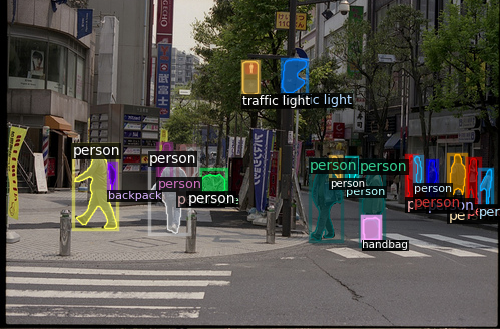
\includegraphics[width=\linewidth]{vis/success/val_848_det.png}
% \end{minipage}
% \begin{minipage}[b]{.49\linewidth}
% 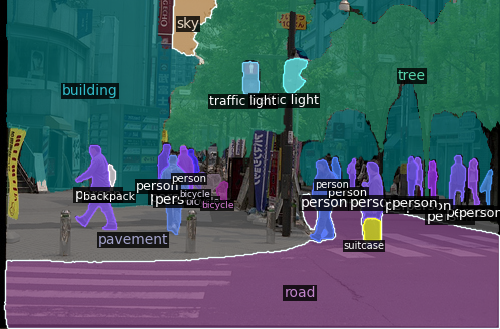
\includegraphics[width=\linewidth]{vis/success/val_848_pan.png}
% \end{minipage}

% \end{minipage}

% \caption{\textbf{Qualitative results} for object detection, segmentation and panoptic segmentation on COCO \val as generated by \ours with ViT-B backbone. \ours can detect and segment objects in crowded scenes.}
% \label{fig:vis}
% % \vspace{-0.2in}
% \end{figure}
% %%%%%%%%%%%%%%%%%%%%%%%%%%%%%%%%%%%%%%%%%%%%%%%%%%%%%%%%%%%%%%%%%%%%

\boldparagraph{Ablation of scale-aware attention.} Here, our baseline is the standard box-attention from \cite{nguyen2022boxer} with single-scale feature input directly taken from the last feature of the ViT backbone (denoted as ``base''). 

From \cref{tab:strat}, we first conclude that \emph{both} scale-aware attention strategies are substantially better than the na\"ive baseline, increasing AP by up to 1.8 points. We note that while fixed-scale attention distributes 25\% of its attention heads into each of the window scales, adaptive-scale attention decides the scale distribution based on the query content. By choosing feature grids from different window scales adaptively, the adaptive-scale attention is able to learn a suitable scale distribution through training data, yielding better performance compared to fixed-scale attention. This is also verified in Fig.~\ref{fig:attn_vis} where queries corresponding to \emph{small} objects tend to pick reference windows of small sizes for its attention heads. Interestingly, queries corresponding to \emph{medium} and \emph{large} objects pick not only reference windows of their sizes, but also ones of smaller sizes. One of reasons may come from the fact that performing instance segmentation of larger objects still requires the network to faithfully preserve the per-pixel spatial details.

In \cref{tab:window_size}, we compare the performance of \ours across several sizes ($s$) of the reference window. They all improve over the baseline, while the choice of a specific base size makes only marginal differences. Our ablation reveals that the number of scales rather than the window size plays an important role to make our network more \emph{scale-aware}. Indeed, in \cref{tab:num_scale}, the use of 4 or more window scales shows improvement up to 0.8 AP over 2 window scales; and clearly outperforms the na\"ive baseline. Last, we show in \cref{tab:feat_scale} that the \emph{decouple} between feature scale and dimension of the ViT backbone and the detection head features helps to boost the performance of our plain detector by $\sim$1 AP point, while keeping its efficiency (\ie, both in terms of FLOPs and FPS). This practice makes scaling of \ours to larger ViT backbones more practical.

\boldparagraph{Ablation on more pre-training data and strategies.} \cref{tab:pretrain} compares the ViT backbone when pre-trained using different strategies with different sizes of pre-training data. \ours with the ViT backbone benefits from better pre-training methods even with supervised approaches. Among supervised pre-training methods, DEiTv3~\cite{touvron2022deit3} shows better results than DEiT~\cite{touvron2021deit}, and the pre-training on more data (\ie, ImageNet-21K) further improves the performance of DEiTv3.
  
However, self-supervised methods like MAE~\cite{he2022mae} provides strong pre-trained backbones when only pre-trained on ImageNet-1K. The best performance is reported with self-supervised method, BEiTv2~\cite{peng2022beitv2} with more pre-training data of ImageNet-21K. This further confirms that our plain detector, \ours, enjoys the significant progress of self-supervised learning and scaling ViTs with data. A similar observation is also pointed out in ViTDet~\cite{li2022vitdet} where the plain ViT backbone initialized with MAE shows better improvement over hierarchical backbones.

%%%%%%%%%%%%%%%%%%%%%%%%%%%%%%%%%%%%%%%%%%%%%%%%%%%%%%%%%%%%%%%%%%%
\begin{table}[t]
    \centering
    \footnotesize
    {
    \tablestyle{7pt}{1.2}
    \begin{tabular}{l|cccc|cccc}
    \multirow{2}{*}{pre-train} & \multicolumn{4}{c|}{Object Detection} & \multicolumn{4}{c}{Instance Segmentation} \\
    & AP$^\text{b}$ & AP$^\text{b}_\text{S}$ & AP$^\text{b}_\text{M}$ & AP$^\text{b}_\text{L}$ & $\text{AP}^\text{m}$ & $\text{AP}^\text{m}_\text{S}$ & $\text{AP}^\text{m}_\text{M}$ & $\text{AP}^\text{m}_\text{L}$ \\
    % \hshline
    % (dynamic)  & \cmark & \xmark & \cmark & \xmark & \cmark & \xmark & \cmark \\
    \shline
    IN-1K, DEiT & 53.6 & 33.7 & 58.1 & 71.5 & 46.1 & 24.5 & 50.4 & 67.2 \\
    IN-1K, DEiTv3 & 54.0 & 34.3 & 58.8 & 70.5 & 46.4 & 24.8 & 51.1 & 66.7 \\
    IN-21K, DEiTv3 & 54.8 & 35.4 & 59.0 & {\bf 72.4} & 47.1 & 25.8 & 51.2 & 68.5 \\
    \hline
    IN-1K, MAE & 55.4 & 36.1 & 59.1 & 70.9 & 47.6 & {\bf 26.8} & 51.4 & 67.1 \\
    IN-21K, BEiTv2 & {\bf 55.7} & {\bf 36.5} & {\bf 60.2} & {\bf 72.4} & {\bf 48.1} & 26.7 & {\bf 52.7} & {\bf 68.9} \\
    % ************************************
    \end{tabular}
    }
    % \vspace{-0.1in}
    % \vspace{-0.5em}
    \caption{
        \textbf{Ablation on scaling with more pre-training data and strategies} of \ours with the plain ViT-B backbone evaluated on COCO object detection and instance segmentation. We compare the plain backbone pre-trained using supervised methods (\emph{top} row) \vs self-supervised methods (\emph{bottom} row) with different sizes of pre-training dataset (ImageNet-1K \vs ImageNet-21K). Here, we use the $5\times$ schedule as in \cite{nguyen2022boxer}. It can be seen that \ours with the plain ViT backbone benefits with more pre-training data (\eg, ImageNet-1K \vs ImageNet-21K) and better pre-training approaches (supervised learning \vs self-supervised learning).
    }\label{tab:pretrain}
    % \vspace{-0.2in}
\end{table}
%%%%%%%%%%%%%%%%%%%%%%%%%%%%%%%%%%%%%%%%%%%%%%%%%%%%%%%%%%%%%%%%%%%%


%%%%%%%%%%%%%%%%%%%%%%%%%%%%%%%%%%%%%%%%%%%%%%%%%%%%%%%%%%%%%%%%%%%%
\begin{figure}[!b]
\centering

\begin{minipage}{1\linewidth}
\centering

\begin{minipage}[b]{.24\linewidth}
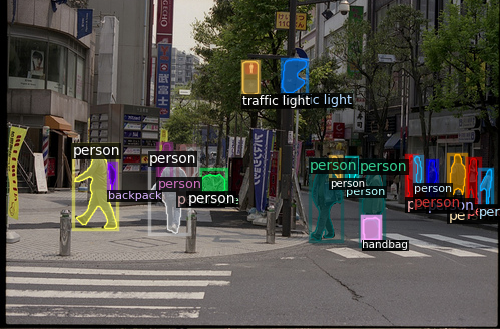
\includegraphics[width=\linewidth]{vis/success/val_848_det.png}
\end{minipage}
\begin{minipage}[b]{.24\linewidth}
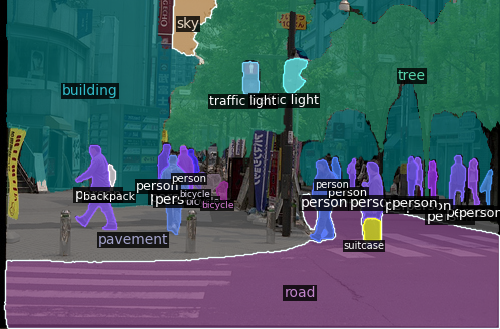
\includegraphics[width=\linewidth]{vis/success/val_848_pan.png}
\end{minipage}
\begin{minipage}[b]{.24\linewidth}
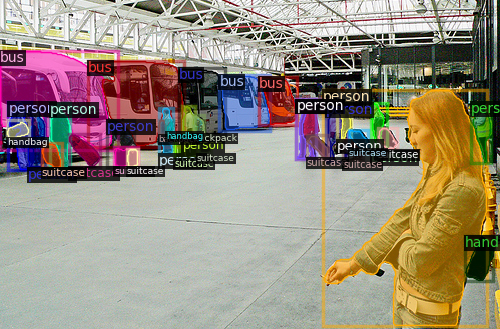
\includegraphics[width=\linewidth]{vis/success/val_965_det.png}
\end{minipage}
\begin{minipage}[b]{.24\linewidth}
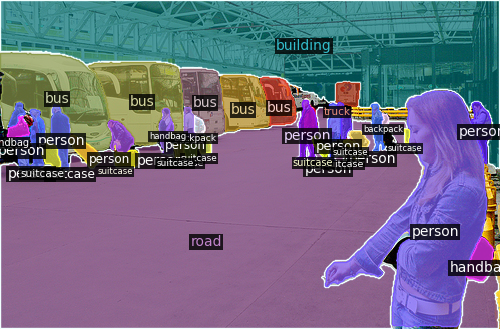
\includegraphics[width=\linewidth]{vis/success/val_965_pan.png}
\end{minipage}

\end{minipage}

\caption{\textbf{Qualitative results} for object detection and panoptic segmentation on the COCO~\cite{lin2014mscoco} 2017 \val set generated by \ours. Note that \ours gives good predictions on \emph{small} objects.}
\label{fig:vis}
% \vspace{-0.2in}
\end{figure}
%%%%%%%%%%%%%%%%%%%%%%%%%%%%%%%%%%%%%%%%%%%%%%%%%%%%%%%%%%%%%%%%%%%%

\boldparagraph{State-of-the-art comparison and scaling behavior.}
We show in \cref{tab:det_main,tab:panoptic} that \ours indicates strong performance on object detection, instance segmentation and panoptic segmentation. To be specific, our plain detector combined with a ViT, pre-trained using MAE \cite{he2022mae} or BEiTv2 \cite{peng2022beitv2}, presents good scaling behavior. When moving to large and huge models, our method outperforms multi-scale counterparts including the recent end-to-end Mask2Former segmentation model \cite{cheng2022mask2former}. Despite involving more advanced attention blocks designs, \ie, shifted window attention in Swin \cite{liu2021swintransformer} and pooling attention in MViT \cite{fan2021mvit}, detectors with hierarchical backbones benefit less from larger backbones. \ours is better than the plain-backbone detector, ViTDet, across all backbones in terms of both accuracy and inference speed.
% The visualization of the \ours prediction can be seen in \cref{fig:vis} (more visualizations are provided in the supplementary).
    
    
    %%%%%%%%%%%%%%%%%%%%%%%%%%%%%%%%%%%%%%%%%%%%%%%%%%%%%%%%%%%%%%%%%%%
    \begin{table}[t]
    \centering
    \footnotesize
    {
    {
    \tablestyle{2.75pt}{1.2}
    \begin{tabular}{lccccccccccc}
    \multicolumn{1}{l|}{\multirow{2}{*}{method}} & \multicolumn{1}{c}{\multirow{2}{*}{backbone}} & \multicolumn{1}{c|}{\multirow{2}{*}{pre-train}} & \multicolumn{4}{c|}{Object Detection} & \multicolumn{4}{c|}{Instance Segmentation} & \multirow{2}{*}{FPS} \\
    \multicolumn{1}{l|}{} & \multicolumn{1}{c}{} & \multicolumn{1}{c|}{} & AP$^\text{b}$ & AP$^\text{b}_\text{S}$ & AP$^\text{b}_\text{M}$ & \multicolumn{1}{c|}{AP$^\text{b}_\text{L}$} & $\text{AP}^\text{m}$ & $\text{AP}^\text{m}_\text{S}$ & $\text{AP}^\text{m}_\text{M}$ & \multicolumn{1}{c|}{$\text{AP}^\text{m}_\text{L}$} &  \\
    % \shline
    % \rowcolor{orange!30} \multicolumn{12}{l}{\footnotesize \textbf{Base models}} \\
    % \multicolumn{1}{l|}{{\color{mygray} Swin~\cite{liu2021swintransformer}}} & {\color{mygray} Swin-B} & \multicolumn{1}{c|}{\color{mygray} sup-22K} & {\color{mygray} 54.0} & {\color{mygray} -} & {\color{mygray} -} & \multicolumn{1}{c|}{{\color{mygray} -}} & {\color{mygray} 46.5} & {\color{mygray} -} & {\color{mygray} -} & \multicolumn{1}{c|}{{\color{mygray} -}} & {\color{mygray} 13} \\
    % \multicolumn{1}{l|}{Mask2Former~\cite{cheng2022mask2former}} & {Swin-B} & \multicolumn{1}{c|}{sup-22K} & \multicolumn{4}{c|}{\small n/a} & \textbf{48.1} & \textbf{27.8} & 52.0 & \multicolumn{1}{c|}{\textbf{71.1}} & {\small -} \\
    % \multicolumn{1}{l|}{{\color{mygray} MViT~\cite{fan2021mvit}}} & {\color{mygray} MViT-B} & \multicolumn{1}{c|}{\color{mygray} sup-22K} & {\color{mygray} 55.6} & {\color{mygray} -} & {\color{mygray} -} & \multicolumn{1}{c|}{{\color{mygray} -}} & {\color{mygray} \textbf{48.1}} & {\color{mygray} -} & {\color{mygray} -} & \multicolumn{1}{c|}{{\color{mygray} -}} & {\color{mygray} 11} \\
    % \multicolumn{1}{l|}{BoxeR~\cite{nguyen2022boxer}} & ViT-B & \multicolumn{1}{c|}{MAE} & 55.4 & - & - & \multicolumn{1}{c|}{-} & 47.7 & - & - & \multicolumn{1}{c|}{-} & 12 \\
    % \multicolumn{1}{l|}{{\color{mygray} ViTDet~\cite{li2022vitdet}}} & {\color{mygray} ViT-B} & \multicolumn{1}{c|}{\color{mygray} MAE} & {\color{mygray} 54.0} & {\color{mygray} 36.5} & {\color{mygray} 57.8} & \multicolumn{1}{c|}{{\color{mygray} 69.1}} & {\color{mygray} 46.7} & {\color{mygray} 27.2} & {\color{mygray} 49.6} & \multicolumn{1}{c|}{{\color{mygray} 64.9}} & {\color{mygray} 11} \\
    % % ************************************
    % \hline
    % \multicolumn{1}{l|}{{\color{mygray} UViT~\cite{chen2022uvit}}} & {\color{mygray} UViT-B} & \multicolumn{1}{c|}{\color{mygray} self-learning} & {\color{mygray} 53.9} & {\color{mygray} -} & {\color{mygray} -} & \multicolumn{1}{c|}{{\color{mygray} -}} & {\color{mygray} 46.1} & {\color{mygray} -} & {\color{mygray} -} & \multicolumn{1}{c|}{{\color{mygray} -}} & {\color{mygray} 12} \\
    % \multicolumn{1}{l|}{{PlainDETR~\cite{lin2023plaindetr}}} & {ViT-B} & \multicolumn{1}{c|}{MAE} & {53.8} & {35.9} & {57.0} & \multicolumn{1}{c|}{{68.9}} & \multicolumn{4}{c|}{\small n/a} & {12} \\
    % \multicolumn{1}{l|}{\ours} & {ViT-B} & \multicolumn{1}{c|}{MAE} & 55.6 & \textbf{37.1} & 59.2 & \multicolumn{1}{c|}{71.5} & 48.0 & {27.5} & 51.5 & \multicolumn{1}{c|}{67.8} & \textbf{15} \\
    % \multicolumn{1}{l|}{\ours} & {ViT-B} & \multicolumn{1}{c|}{BEiTv2} & \textbf{55.7} & {36.5} & \textbf{60.2} & \multicolumn{1}{c|}{\textbf{72.3}} & \textbf{48.1} & {26.7} & \textbf{52.7} & \multicolumn{1}{c|}{{68.9}} & \textbf{15} \\
    % % ************************************
    \shline
    \rowcolor{orange!50} \multicolumn{12}{l}{\footnotesize \textbf{Feature pyramids}} \\
    % \multicolumn{1}{l|}{{\color{mygray} Swin~\cite{liu2021swintransformer}}} & {\color{mygray} Swin-L} & \multicolumn{1}{c|}{\color{mygray} sup-22K} & {\color{mygray} 54.8} & {\color{mygray} -} & {\color{mygray} -} & \multicolumn{1}{c|}{{\color{mygray} -}} & {\color{mygray} 47.3} & {\color{mygray} -} & {\color{mygray} -} & \multicolumn{1}{c|}{{\color{mygray} -}} & {\color{mygray} \textbf{10}} \\
    % \multicolumn{1}{l|}{Mask2Former~\cite{cheng2022mask2former}} & {Swin-L} & \multicolumn{1}{c|}{sup-22K} & \multicolumn{4}{c|}{\small n/a} & 50.1 & 29.9 & 53.9 & \multicolumn{1}{c|}{\textbf{72.1}} & 4 \\
    % \multicolumn{1}{l|}{{\color{mygray} MViT~\cite{fan2021mvit}}} & {\color{mygray} MViT-L} & \multicolumn{1}{c|}{\color{mygray} sup-22K} & {\color{mygray} 55.7} & {\color{mygray} -} & {\color{mygray} -} & \multicolumn{1}{c|}{{\color{mygray} -}} & {\color{mygray} 48.3} & {\color{mygray} -} & {\color{mygray} -} & \multicolumn{1}{c|}{{\color{mygray} -}} & {\color{mygray} 6} \\
    % \multicolumn{1}{l|}{{\color{mygray} ViTDet~\cite{li2022vitdet}}} & {\color{mygray} ViT-L} & \multicolumn{1}{c|}{\color{mygray} MAE} & {\color{mygray} 57.6} & {\color{mygray} 40.5} & {\color{mygray} 61.6} & \multicolumn{1}{c|}{{\color{mygray} 72.6}} & {\color{mygray} 49.9} & {\color{mygray} 30.5} & {\color{mygray} 53.3} & \multicolumn{1}{c|}{{\color{mygray} 68.0}} & {\color{mygray} 7} \\
    \multicolumn{1}{l|}{{Swin~\cite{liu2021swintransformer}}} & {Swin-L} & \multicolumn{1}{c|}{sup-21K} & {55.0} & {38.3} & {59.4} & \multicolumn{1}{c|}{{71.6}} & {47.2} & {28.7} & {50.5} & \multicolumn{1}{c|}{{66.0}} & {10} \\
    \multicolumn{1}{l|}{Mask2Former~\cite{cheng2022mask2former}} & {Swin-L} & \multicolumn{1}{c|}{sup-21K} & \multicolumn{4}{c|}{\small n/a} & 50.1 & 29.9 & 53.9 & \multicolumn{1}{c|}{\textbf{72.1}} & 4 \\
    \multicolumn{1}{l|}{{MViT~\cite{fan2021mvit}}} & {MViT-L} & \multicolumn{1}{c|}{sup-21K} & {55.7} & {40.3} & {59.6} & \multicolumn{1}{c|}{{71.4}} & {48.3} & {31.1} & {51.2} & \multicolumn{1}{c|}{{66.3}} & {6} \\
    \multicolumn{1}{l|}{{ViTDet~\cite{li2022vitdet}}} & {ViT-L} & \multicolumn{1}{c|}{MAE} & {57.6} & {40.5} & {61.6} & \multicolumn{1}{c|}{{72.6}} & {49.9} & {30.5} & {53.3} & \multicolumn{1}{c|}{{68.0}} & {7} \\
    % ************************************
    \hline
    % \multicolumn{1}{l|}{{\color{mygray} MViT~\cite{li2022vitdet}}} & {\color{mygray} MViT-H} & \multicolumn{1}{c|}{\color{mygray} sup-22K} & {\color{mygray} 55.7} & {\color{mygray} -} & {\color{mygray} -} & \multicolumn{1}{c|}{{\color{mygray} -}} & {\color{mygray} 48.3} & {\color{mygray} -} & {\color{mygray} -} & \multicolumn{1}{c|}{{\color{mygray} -}} & {\color{mygray} 6} \\
    % \multicolumn{1}{l|}{{\color{mygray} ViTDet~\cite{li2022vitdet}}} & {\color{mygray} ViT-H} & \multicolumn{1}{c|}{\color{mygray} MAE} & {\color{mygray} 58.7} & {\color{mygray} 41.9} & {\color{mygray} 63.0} & \multicolumn{1}{c|}{{\color{mygray} 73.9}} & {\color{mygray} 50.9} & {\color{mygray} 32.0} & {\color{mygray} 54.3} & \multicolumn{1}{c|}{{\color{mygray} 68.9}} & {\color{mygray} 5} \\
    \multicolumn{1}{l|}{{MViT~\cite{li2022vitdet}}} & {MViT-H} & \multicolumn{1}{c|}{sup-21K} & {55.9} & {40.8} & {59.8} & \multicolumn{1}{c|}{{70.8}} & {48.3} & {30.1} & {51.1} & \multicolumn{1}{c|}{{66.6}} & {6} \\
    \multicolumn{1}{l|}{{ViTDet~\cite{li2022vitdet}}} & {ViT-H} & \multicolumn{1}{c|}{MAE} & {58.7} & {41.9} & {63.0} & \multicolumn{1}{c|}{{73.9}} & {50.9} & {32.0} & {54.3} & \multicolumn{1}{c|}{{68.9}} & {5} \\
    % ************************************
    \shline
    \rowcolor{orange!50} \multicolumn{12}{l}{\footnotesize \textbf{Plain features}} \\
    \multicolumn{1}{l|}{\ours} & {ViT-L} & \multicolumn{1}{c|}{MAE} & {58.5} & {42.2} & {62.5} & \multicolumn{1}{c|}{{73.4}} & 50.6 & {32.1} & {54.2} & \multicolumn{1}{c|}{69.8} & 9 \\
    \multicolumn{1}{l|}{\ours} & {ViT-L} & \multicolumn{1}{c|}{BEiTv2} & {58.7} & {40.4} & {63.2} & \multicolumn{1}{c|}{{74.8}} & {50.9} & {30.4} & {55.1} & \multicolumn{1}{c|}{70.9} & 9 \\
    % ------------------------------------------------------------------------------------------------
    \hline
    \multicolumn{1}{l|}{\ours} & {ViT-H} & \multicolumn{1}{c|}{MAE} & \textbf{59.8} & \textbf{42.2} & \textbf{63.8} & \multicolumn{1}{c|}{\textbf{74.9}} & \textbf{51.9} & \textbf{32.2} & \textbf{55.7} & \multicolumn{1}{c|}{{71.0}} & 7 \\
    \end{tabular}
    }
    }
    % \vspace{1em}
    \caption{\textbf{State-of-the-art comparison and scaling behavior for object detection and instance segmentation.} We compare methods using feature pyramids \vs plain features on COCO \val (n/a: entry is not available). Backbones with MAE pre-trained on ImageNet-1K while others pre-trained on ImageNet-21K. 
    % \ours indicates good scaling behavior. 
    With only single-scale features, \ours shows strong performance compared to multi-scale detectors including transformer-based detectors like Mask2Former, while being $\sim2\times$ faster.}
    \label{tab:det_main}
    % \vspace{-0.2in}
    \end{table}
    %%%%%%%%%%%%%%%%%%%%%%%%%%%%%%%%%%%%%%%%%%%%%%%%%%%%%%%%%%%%%%%%%%%%

    \begin{table}[t]
        \centering
        \footnotesize
        {
        \tablestyle{3.25pt}{1.2}
        \begin{tabular}{lcccccc}
        \multicolumn{1}{l|}{\multirow{2}{*}{method}} & \multirow{2}{*}{backbone} & \multicolumn{1}{c|}{\multirow{2}{*}{pre-train}} & \multicolumn{3}{c|}{Panoptic Segmentation} & \multirow{2}{*}{FPS} \\
        \multicolumn{1}{l|}{} &  & \multicolumn{1}{c|}{} & PQ & PQ$^\text{th}$ & \multicolumn{1}{c|}{PQ$^\text{st}$} & \\
        \shline
        \rowcolor{orange!50} \multicolumn{7}{l}{\footnotesize \textbf{Feature pyramids}} \\
        \multicolumn{1}{l|}{MaskFormer~\cite{cheng2021maskformer}} & Swin-B & \multicolumn{1}{c|}{sup-21K} & 51.8 & 56.9 & \multicolumn{1}{c|}{44.1} & - \\
        \multicolumn{1}{l|}{Mask2Former~\cite{cheng2022mask2former}} & Swin-B & \multicolumn{1}{c|}{sup-21K} & 56.4 & 62.4 & \multicolumn{1}{c|}{47.3} & - \\
        \hline
        \multicolumn{1}{l|}{Mask2Former~\cite{cheng2022mask2former}} & Swin-L & \multicolumn{1}{c|}{sup-21K} & 57.8 & 64.2 & \multicolumn{1}{c|}{48.1} & 4 \\
        \shline
        \rowcolor{orange!50} \multicolumn{7}{l}{\footnotesize \textbf{Plain features}} \\
        \multicolumn{1}{l|}{\ours} & ViT-B & \multicolumn{1}{c|}{BEiTv2} & {56.5} & {62.6} & \multicolumn{1}{c|}{{47.3}} & {13} \\
        \hline
        \multicolumn{1}{l|}{\ours} & ViT-L & \multicolumn{1}{c|}{BEiTv2} & \textbf{58.5} & \textbf{65.1} & \multicolumn{1}{c|}{\textbf{48.6}} & {8} \\
        \end{tabular}
        }
        % \vspace{1em}
        {\caption{\textbf{State-of-the-art comparison and scaling behavior for panoptic segmentation.} We compare between methods using feature pyramids (\emph{top} row) \vs single-scale (\emph{bottom} row) on COCO~\val. \ours with single-scale input shows better results when scaling to larger backbones, while being $\sim2\times$ faster compared to Mask2Former.}\label{tab:panoptic}}%
    \end{table}

    \boldparagraph{Limitations.} Our final goal is to simplify the detection pipeline and to achieve competitive results at the same time. In \cref{sec:experiments}, we find that the \emph{adaptive-scale} attention mechanism that adaptively learns scale-aware information in its computation plays a key role for a plain detector. However, our adaptive-scale attention still encodes the knowledge of different scales. In the future, we hope that with the large-scale training data, a simpler design of the attention mechanism could also learn the scale equivariant property. Furthermore, \ours faces difficulties in detecting and segmenting large objects in the image. To overcome this limitation, we think that a design of attention computation which effectively combines both global and local information is necessary.
